\chapter{Anexo I: Matriz de Consistencia}

% Incluye la imagen de la primera parte de la matriz
\begin{figure}[h!]
	\centering
	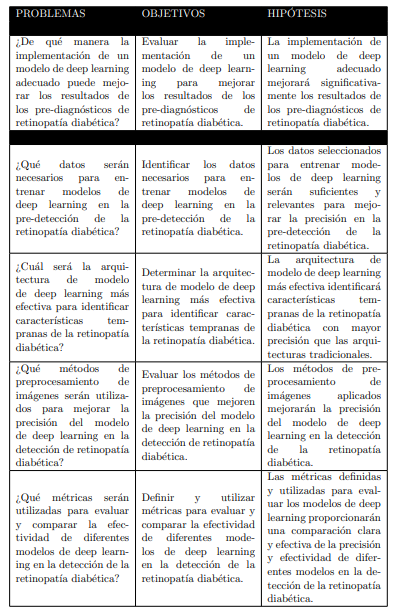
\includegraphics[width=\textwidth]{C:/Users/José Arroyo/Desktop/tesis cambios/TesisJoseArroyo/images_repo/MATRIZ PARTE 1.png}
	\caption{Matriz de consistencia (Parte 1). Fuente: Elaboración propia}
	\label{fig:matriz_parte1}
\end{figure}

% Incluye la imagen de la segunda parte de la matriz
\begin{figure}[h!]
	\centering
	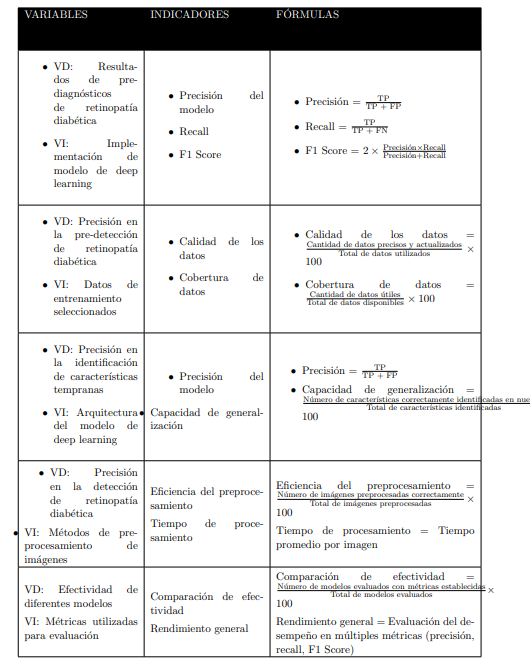
\includegraphics[width=\textwidth]{C:/Users/José Arroyo/Desktop/tesis cambios/TesisJoseArroyo/images_repo/MATRIZ PARTE 2.png}
	\caption{Matriz de consistencia (Parte 2). Fuente: Elaboración propia}
	\label{fig:matriz_parte2}
\end{figure}

\chapter{Anexo II: Árbol de Problemas}

% Incluye la imagen del árbol de problemas
\begin{figure}[h!]
	\centering
	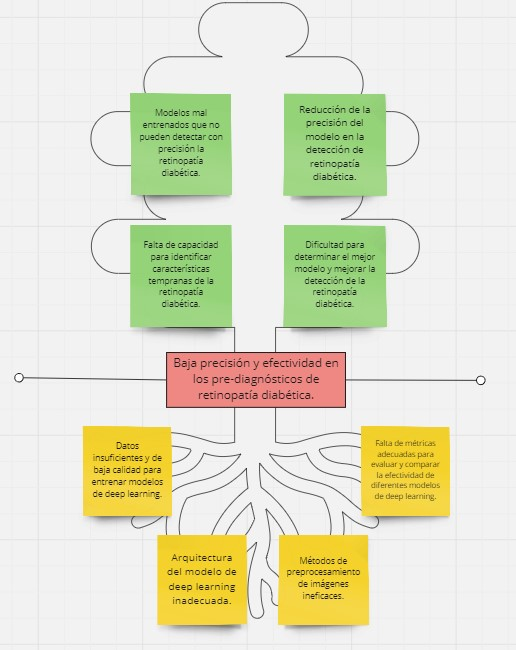
\includegraphics[width=\textwidth]{C:/Users/José Arroyo/Desktop/tesis cambios/TesisJoseArroyo/images_repo/Arbol de problemas miro.jpg}
	\caption{Árbol de Problemas. Fuente: Elaboración propia}
	\label{fig:arbol_problemas}
\end{figure}

\chapter{Anexo III: Resumen de Papers Investigados}

\begin{table}[h!]
	\centering
	\footnotesize
	\begin{tabular}{|p{0.5cm}|p{0.3cm}|p{4cm}|p{2cm}|p{0.6cm}|p{1.7cm}|p{3cm}|}
		\hline
		\rowcolor{bluejean} \multicolumn{1}{|c|}{\textcolor{white}{Tipo}} & \multicolumn{1}{c|}{\textcolor{white}{N°}} & \multicolumn{1}{c|}{\textcolor{white}{Título}} & \multicolumn{1}{c|}{\textcolor{white}{Autor}} & \multicolumn{1}{c|}{\textcolor{white}{Año}} & \multicolumn{1}{c|}{\textcolor{white}{País}} & \multicolumn{1}{c|}{\textcolor{white}{Fuente}} \\
		\hline
		\multirow{2}{*}{\rotatebox[origin=c]{90}{Problema}} & 1 & Deep Convolutional Neural Networks for Detecting COVID-19 Using Medical Images: A Survey & Sharma, et al. & 2020 & India & \textit{IEEE Access} \\
		\cline{2-7}
		& 2 & Heart Disease Detection Using Machine Learning and Deep Learning Techniques & Jiang, et al. & 2020 & USA & \textit{International Journal of Medical Informatics} \\
		\hline
		\multirow{3}{*}{\rotatebox[origin=c]{90}{Propuesta}} & 3 & Monitoring and Recognition of Heart Health using Heartbeat Classification with Deep Learning and IoT & Arulkumar, et al. & 2023 & India & \textit{Journal of Machine and Computing} \\
		\cline{2-7}
		& 4 & Advances in Deep Learning: From Diagnosis to Treatment & Huang, et al. & 2023 & China & \textit{BioScience Trends} \\
		\cline{2-7}
		& 5 & A Study on Scope of Artificial Intelligence in Diagnostic Medicine & Santhosh Kumar, et al. & 2023 & India & \textit{IEEE Access} \\
		\hline
		\multirow{3}{*}{\rotatebox[origin=c]{90}{Otros}} & 6 & A Diabetic Retinopathy Detection using Customized Convolutional Neural Network & Mane, et al. & 2023 & India & \textit{International Journal of Electrical and Electronics Research} \\
		\cline{2-7}
		& 7 & Using Deep Learning Architectures for Detection and Classification of Diabetic Retinopathy & Mohanty, et al. & 2023 & India & \textit{Sensors} \\
		\cline{2-7}
		& 8 & Prevalencia de la retinopatía diabética y factores de riesgo asociados & Yáñez, et al. & 2016 & Peru & \textit{Revista Médica Carrionica} \\
		\hline
	\end{tabular}
	\caption{Cuadro Resumen de Papers Investigados. Fuente: Elaboración propia}
	\label{A:table}
\end{table}

\end{document}
